%\documentclass[prb,aps,showpacs,twocolumn,nofootinbib]{revtex4}
\documentclass[prb,aps,showpacs,preprint,nofootinbib]{revtex4}

%\usepackage{txfonts}
\usepackage[dvipdfmx]{graphicx}% Include figure files
\usepackage{dcolumn}% Align table columns on decimal point
\usepackage{bm}% bold math
\usepackage{color}
\usepackage{ulem}
\usepackage{amsfonts,amsthm}
\usepackage{amsmath}
\usepackage{amssymb}
\usepackage{algorithm}
\usepackage{algorithmic}
%\usepackage{cite}
%\usepackage{amsfonts,amsthm}

%\documentclass[twocolumn,amsmath,amssymb]{kotaibuturi} 

%\def\theequation{\arabic{section}.\arabic{equation}}
%%%%%%%%%%%%%%%%%%%%%%%%%%%%%%%%%%%%%%%%%%%%%%%%%%%%%%%%%%%%%%
%\pagestyle{empty}
%\usepackage{bm} 
%\usepackage{enumerate}
%\usepackage{graphicx,color}%  
%\usepackage{amsmath,amsfonts,amsthm,amssymb,slashbox} 
%\usepackage{dcolumn}
%\usepackage{ulem}
 
 
%\setlength{\textwidth}{16.6cm} 
%\setlength{\textheight}{21.8cm} 
%\setlength{\oddsidemargin}{+2.5cm} 
\setlength{\topmargin}{-1.0cm} 
\def\etal{{\itshape et al.}}
\def\journal#1#2#3#4{#1 {\bf #2} (#4) #3}
\def\JPSJ{J.\ Phys.\ Soc.\ Jpn.}
\def\PR{Phys.\ Rev.}
\def\PRL{Phys.\ Rev.\ Lett.}
\def\PRB{Phys.\ Rev.\ B}
\def\PRD{Phys.\ Rev.\ D}
\def\RMP{Rev.\ Mod.\ Phys.}
\def\JCP{J.\ Chem.\ Phys.}
\makeatletter
\def\widebar{\accentset{\overline{\mskip12mu}}}
\makeatother
%--------------------------------------------------------
%------------------------------------
\newcommand{\bchi}{\mbox{\boldmath $\chi$}} 
\newcommand{\bE}{\mbox{\boldmath $E$}} 
\newcommand{\bD}{\mbox{\boldmath $D$}} 
\newcommand{\bK}{\mbox{\boldmath $K$}} 
\newcommand{\bQ}{\mbox{\boldmath $Q$}} 
\newcommand{\bF}{\mbox{\boldmath $F$}} 
\newcommand{\bH}{\mbox{\boldmath $H$}} 
\newcommand{\bG}{\mbox{\boldmath $G$}} 
\newcommand{\bC}{\mbox{\boldmath $C$}} 
\newcommand{\bZ}{\mbox{\boldmath $Z$}} 
\newcommand{\bmu}{\mbox{\boldmath $\mu$}} 
\newcommand{\bu}{\mbox{\boldmath $u$}} 
\newcommand{\bq}{\mbox{\boldmath $q$}} 
\newcommand{\br}{\mbox{\boldmath $r$}} 
\newcommand{\bR}{\mbox{\boldmath $R$}} 
\newcommand{\bk}{\mbox{\boldmath $k$}} 
\newcommand{\bOmega}{\mbox{\boldmath $\Omega$}}
\newcommand{\btau}{\mbox{\boldmath $\tau$}}  
\newcommand{\bO}{\mbox{\boldmath $O$}} 
\newcommand{\bS}{\mbox{\boldmath $S$}}
\newcommand{\lef}{\leftarrow}
\newcommand{\Lef}{\Leftarrow}
\newcommand{\up}{\uparrow}
\newcommand{\down}{\downarrow}
%
%
\newcommand{\bdot}{\bm{\cdot}}
%
\newcommand{\Ha}{\mathcal{H}}
\newcommand{\mh}{\mathsf{h}}
\newcommand{\mA}{\mathsf{A}}
\newcommand{\mB}{\mathsf{B}}
\newcommand{\mC}{\mathsf{C}}
\newcommand{\mS}{\mathsf{S}}
\newcommand{\mU}{\mathsf{U}}
\newcommand{\mX}{\mathsf{X}}
\newcommand{\sP}{\mathcal{P}}
\newcommand{\sL}{\mathcal{L}}
\newcommand{\sO}{\mathcal{O}}
\newcommand{\sH}{\mathcal{H}}
%
\newcommand{\HPhi}{\mathcal{H}\Phi}
\newcommand{\Pf}{\mathrm{Pf}\,}
\newcommand{\Tr}{\mathrm{Tr}\,}
%
\newcommand{\ep}{\varepsilon}
%
\newcommand{\Ns}{N_{\text{s}}}

\renewcommand{\figurename}{図}

\arraycolsep=0.2em 
 
%-------------------------------- 
\setlength{\textwidth}{504pt} 
\setlength{\columnsep}{14pt} 
\hoffset-23.5pt 
%-------------------------------- 

\newcommand{\tr}[1]{\textcolor{red}{#1}}
\newcommand{\txtrout}[1]{\textcolor{red}{\sout{#1}}}
\newcommand{\tb}[1]{\textcolor{blue}{#1}}
\newcommand{\txtbout}[1]{\textcolor{blue}{\sout{#1}}}
\newcommand{\tg}[1]{\textcolor{magenta}{#1}}
\newcommand{\txtgout}[1]{\textcolor{magenta}{\sout{#1}}}

%
%
\newcommand{\la}{\langle}
\newcommand{\ra}{\rangle}
\newcommand{\ga}{\alpha}
\newcommand{\gb}{\beta}
\newcommand{\gc}{\gamma}
\newcommand{\gs}{\sigma}
\newcommand{\vk}{{\bm{k}}}
\newcommand{\vq}{{\bm{q}}}
%\newcommand{\vr}{{\bm{r}}}
\newcommand{\vR}{{\bm{R}}}
\newcommand{\vQ}{{\bm{Q}}}
\newcommand{\vga}{{\bm{\alpha}}}
\newcommand{\vgc}{{\bm{\gamma}}}
\newcommand{\mb}[1]{\mathbf{#1}}
\def\vec#1{\boldsymbol #1}
\arraycolsep=0.0em




%
% lengths
%
%\setlength{\topmargin}{-10mm}
%\setlength{\headsep}{8mm}
%\setlength{\oddsidemargin}{-10mm}
%\setlength{\evensidemargin}{-10mm}
%\setlength{\textwidth}{18cm}
%\setlength{\textheight}{23.5cm}
%\setlength{\baselineskip}{1.8zh}
%\setlength{\parindent}{1zw}
%\setlength{\parskip}{0.1\baselineskip}
%\renewcommand{\baselinestretch}{1.0}




\begin{document}
\begin{center}\LARGE
$\mathcal H\Phi$におけるいくつかの工夫
\end{center}
\begin{flushright}\large
三澤 貴宏 \\
東京大学物性研究所計算物質科学研究センター
\end{flushright}

\section{はじめに}
\label{sec:intro}
厳密対角化、とくにLanczos法を用いた大規模計算を
行なう上での計算上の幾つかの工夫を解説する。
行列要素が全て確保できない位巨大になってくると、
行列要素を逐次生成しながら行列-ベクトル積の計算を
行なうことになるが、その計算量は莫大に
なるので、計算コストを削減するために
様々な工夫を行なうことになる。
TITPACK ver.2~\cite{titpack}およびそのマニュアルは
その工夫をどう行なうかを明確に解説してあり、
その後の対角化のコードを作成する人にとって
大きな参考となってきた。
この解説では、TITPACKで用いている工夫に付け加えて、
$\HPhi$で用いている工夫について解説する。

\section{記法などについて}
この説明では、
spin 1/2の系を例にとって説明を行なう。
$S^{z}$成分を対角にする表示をとることで、
Hilbert空間の全ての要素を実空間配置に
とることができる。
例えば、$|\up,\up,\up,\down\rangle$などは
$\up$=1, $\down$ =0とすれば,
2進数で[1110]と表すことができる。
14=[1110]とすることで、
状態を2進数表示すなわちbitで表現できる。
交換項などはbitの入れ替えとして
bit演算を用いることで計算を
効率的に行なうことができる。
また、Hubbard模型でも同様に表現が行える。
Hubbard模型の場合は
up,downの電子をそれぞれ0,1で表現することで、
2進数で表せる。
例えば, $|\up\down,\up,\down,0\rangle$
は[11,10,01,00]と表せる。


\section{Hilbert空間の制限について}
\subsection{2次元サーチ法}
\label{sec:OgataLin}
これは、TITPACKで用いられている基本的な方法であり、
Hilbert空間を制限した場合にその逆引きを
効率よく行なう方法である。まずは、この方法を解説する。
例えば、total$S^z$が一定の空間で考える場合は、
前実空間配置の中から、指定したtotal
$S^z$を持つものを抜き出して、
一つ一つlistに格納して行けばよい。
問題はある実空間配置が制限したHilbert空間の中で、
何番目の要素なのかを
逆引きする場合である。
一番、愚直な実装は全ての実空間要素に対して逆引きのリスト
もっておくこと
だがこれはあまりにもコストが大きすぎる。
この逆引きを効率よく
おこなうのが2次元サーチ法である~\cite{Lin,titpack}。

\begin{figure}[h!]
        \begin{center}
                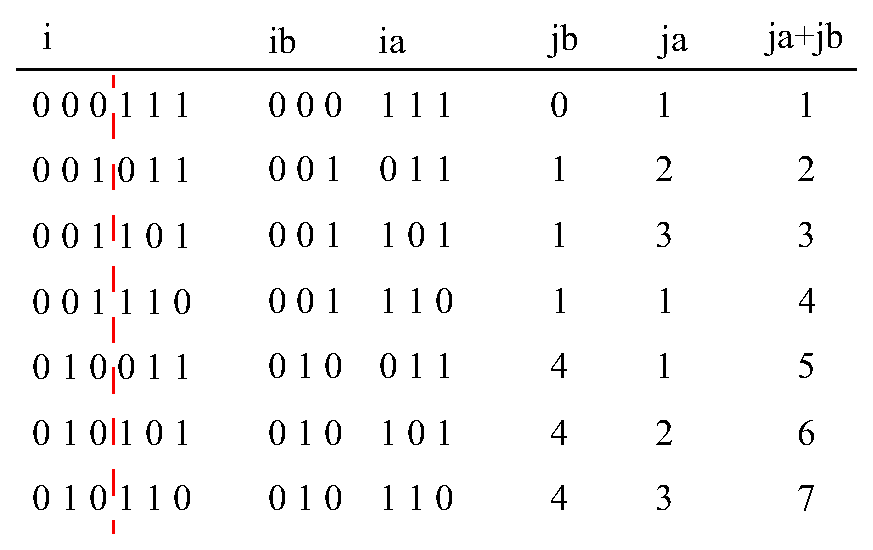
\includegraphics[width=12cm,clip]{2DSearch.eps}
        \end{center}
\caption{2次元サーチ法の図。
iのbitを2つに分割して、分割したbitの情報から、何番目の要素かを
再現する方法。}
\label{fig:2DSearch}
\end{figure}


\begin{algorithm}                      
\caption{Two-dimensional search}         
\begin{algorithmic}                  
\STATE jb$\lef 0$, ja$\lef 0$, icnt$\lef 0$, ib\_old $\lef 0$
\FOR{i=0 to $2^{\rm N}$-1}
\IF{ number of bit in i = Nup}
\STATE list\_1[icnt] $\lef$ i
\STATE ib $\lef$ get\_ib(i)~~~~~~~~~~~~~~~~~//get ib from i
\STATE ia $\lef$ get\_ia(i)~~~~~~~~~~~~~~~~~//get ia from i
  \IF{ ib = ib\_old}
  \STATE ja $\lef$ ja+1
  \ELSE
  \STATE ib\_old $\lef$ ib
  \STATE ja $\lef$ 1
  \STATE jb $\lef$ icnt-1
  \ENDIF
\STATE  list\_ja[ia] $\lef$ ja
\STATE  list\_jb[ib] $\lef$ jb
\STATE  icnt $\lef$ icnt+1
\ENDIF
\ENDFOR
\end{algorithmic}
\label{alg:2DSearch}
\end{algorithm}



この方法の肝は2進表示した状態のbit
を2つに分割することにある(これが2次元サーチ法の名前の由来)。
図\ref{fig:2DSearch}に6site, $S^{z}=0$の場合を示している。
この場合、iを2つに分割した、
上位bitがib,下位bitがiaである。
jb, jaは以下のルールで逐次的に決めていく。
\begin{enumerate}
\item 最初はjb=0, ja=1
\item ibが変化しないなら、jbはそのままでjaを1つずつ増やしていく
\item ibが変化したときは、jaを1にして、jbはひとつ前のja+jbの値にする
\end{enumerate}
こうしておけば、ja+jbがiが何番目かの要素を示すようになる。
それぞれのib, iaに対して、jb, jaは一意に決めるので、
list\_jb[ib], list\_ja[ia]
という2つの配列(配列の大きさは$2^(N/2)$なので小さい)
をもっておけば、iからja+jbを生成することができるようになる。

2次元サーチ法のアルゴリズムの擬似コードを
{\bf Algorithm}~\ref{alg:2DSearch}に示す。
例としてN siteのspin-1/2の系を想定している。
また,total$S^z=$Nupとしている(つまり,1のbitの個数がNup)。
list\_1は要件をみたす(つまり所定の$S^{z}$を満たす)
Hilbert空間の元を
格納する配列であり、get\_ib,get\_iaは
それぞれiから上位bit ib,下位bit iaをとり出す関数である。

\newpage
\subsection{2次元サーチ法のスレッド並列化について}
\label{sec:thread}

\begin{algorithm}                      
\caption{Parallelization for two-dimensional search algorithm}         
\label{alg1}                          
\begin{algorithmic}                  
\STATE jb$\lef 0$
\FOR{ib=0 to $2^{\rm N/2}$-1}
  \STATE list\_jb[ib] $\lef$ ib
  \STATE ib\_Nup $\lef$ count\_bit(ib)
  \STATE jb $\lef$ jb+Binomial(N/2,Nup-ib\_Nup)
\ENDFOR
\FOR{ib=0 to $2^{\rm N/2}$-1}
  \STATE jb $\lef$ list\_jb[ib]
  \STATE ib\_Nup $\lef$ count\_bit(ib)
  \STATE ja $\lef$ 1 
  \FOR{ia=0 to $2^{\rm N/2}$-1}
    \STATE ia\_Nup = count\_bit(ia)
    \IF{ib\_Nup+ia\_Nup=Nup}
      \STATE list\_1[ja+jb] $\lef$ ia+ib*ihfbit
      \STATE list\_ja[ia] $\lef$ ja
      \STATE list\_jb[ib] $\lef$ jb
      \STATE js $\lef$ ja+1
    \ENDIF
  \ENDFOR
\ENDFOR
\end{algorithmic}
\label{alg:P2DSearch}
\end{algorithm}

さて、次は2次元サーチ法のアルゴリズムの
並列化について述べる。
逐次的な操作が入ってしまっているので、
通常は並列化が不可能なように見えるが、
ループをib,iaに関するループに分割することで、
並列計算が可能である。
まず, 2次元サーチののアルゴリズムからib,iaの
ループを入れ子にすることが可能であす。
ibで外側のループを回し、iaで内側のループ
を回せばよい。
そして、ibに依る部分がjbだけだというところが
味噌である。
ibとjbは一対一に対応するので、
ibに対応するjbがわかれば、
ibに関するループは独立に計算でき、
並列計算が行える。
ibに対応するjbは
ibに対応するiaの数を
二項係数を計算することで、
前もって知ることができる。
このibに関するループの部分は並列化不可能だが
ループ長が$2^{N/2}$なので、
この部分の計算時間は実質無視できる。
そのあとで、ib,iaの入れ子のループで
外側のibのループをopenmpでthread並列化
すればよい。

擬似コードを{\bf Algorithme}~\ref{alg:P2DSearch}に
示す。ib,iaの1のbitの個数を数える関数(count\_bit)と
二項係数を計算する関数(Binomial)が必要だが、
それ以外はもとの2次元サーチ法のアルゴリズムと
同じである。また、ihfbit=$2^{N/2}$でia,ibから
もとのiを復元するために必要な数である。

\newpage
\subsection{同じ1のbitの個数をもつ次のbitを生成する方法}
\label{sec:snoob}
2次元サーチ法の並列化のアルゴリズム
をみると、並列化はされるが全体のループ長
は依然として$2^{N}$で計算コストのオーダーは
変わっていないことがわかる。
実はこの計算コストを縮めることも可能である。
鍵となるアルゴリズムは
「ある数と同じ1のbitの個数を持つ数のなかで次に
大きい数を求める方法」
である。
これは「ハッカーの楽しみ」~\cite{hacker}という本に乗っている方法
である~\footnote{この本の作者はこのアルゴリズムの紹介の前に、
「いったい誰がそんなものを計算したがるのか
という疑問が生じる」といっているが、
実際に役に立つ例がここにあった!}
%アルゴリズムの詳細はその本に譲るが、
このアルゴリズムの擬似コードを{\bf Algorithm}~\ref{alg:snoob}
にのせる。
注意しなければならないのはxが0より大きくある必要
がある必要があるということである。
わずか、6行で次の数が生成できる華麗な
アルゴリズムである。

\begin{algorithm}                      
\caption{snoob: Get next larger bit}         
\begin{algorithmic}                  
\STATE smallest $\lef$ x $\&$ (-x)
\STATE ripple $\lef$ x $+$ smallest
\STATE ones $\lef$ x \^\ ripple
\STATE ones $\lef$ (ones $>>$ 2)/smallest
\STATE next\_x $\lef$ ripple $|$ ones
\end{algorithmic}
\label{alg:snoob}                          
\end{algorithm}


\subsection{さらなるスレッド並列化について}
\label{sec:thread}
「ハッカーの楽しみ」の方法を
用いて、さらなる効率化をしてみよう。
まず、最初の2次元サーチ法のアルゴリズムそのものに
この方法をつかってもよいがそれだと
並列化はできない。
並列化バージョンに対して、iaのループの部分で
「ハッカーの楽しみ」の方法を
使うのことで並列化ができる。

Algorithm\ref{alg:PHack}に
擬似コードを示す。
基本は2次元サーチ法の並列化版と
同じでiaのループに関してのみ、
snoobを用いている。
snoobは0には使えないことに注意してほしい。
これによって、計算コストは
減少して、
%2$^N$から
%2$^(N/2)$$\times$まで、
おちてN=36といった巨大な系でも
ヒルベルト空間作成のコストは
ほぼ0になる。
また、飽和磁場近傍の
サイズ自体は大きいが、
状態数が少ないところの
計算も行えるようになっている。
例えば、48サイト2up,46downと
いった条件のヒルベルト空間の作成はすぐに行える。

\begin{algorithm}                      
\caption{Parallelization for 2D search algorithm II}         
\label{alg:PHack}                          
\begin{algorithmic}                  
\STATE jb$\lef 0$
\FOR{ib=0 to $2^{\rm N/2}$-1}
  \STATE list\_jb[ib] $\lef$ ib
  \STATE ib\_Nup $\lef$ count\_bit(ib)
  \STATE jb $\lef$ jb+Binomial(N/2,Nup-ib\_Nup)
\ENDFOR
\FOR{ib=0 to $2^{\rm N/2}$-1}
  \STATE jb $\lef$ list\_jb[ib]
  \STATE ib\_Nup $\lef$ count\_bit(ib)
  \STATE ja $\lef$ 1 
    \IF{ib\_Nup $\leq$ Nup}
      \STATE ia = 2$^{\rm Nup-ib\_Nup}$-1
      \IF{ia $<$  ihfbit}
        \STATE list\_1[ja+jb] $\lef$ ia+ib*ihfbit
        \STATE list\_ja[ia] $\lef$ ja
        \STATE list\_jb[ib] $\lef$ jb
        \STATE ja $\lef$ ja+1
        \IF{ia $\neq$ 0}
          \STATE ia $\lef$ snoob(ia)
          \WHILE{ia $<$ ihfbit}
             \STATE list\_1[ja+jb] $\lef$ ia+ib*ihfbit
             \STATE list\_ja[ia] $\lef$ ja
             \STATE list\_jb[ib] $\lef$ jb
             \STATE ja $\lef$ ja+1
             \STATE ia $\lef$ snoob(ia)
          \ENDWHILE
        \ENDIF
      \ENDIF
    \ENDIF
\ENDFOR
\end{algorithmic}
\end{algorithm}

\newpage

\section{Fermionサインの数え方について}
ハバード模型など遍歴電子系の
フェルミオンサインについて説明する。
つねに粒子がいるスピン系とは違い、
遍歴電子系の場合は電子がいないサイトが
あるので、ホッピング項などを
作用させるときにフェルミオンの
交換関係から符号が生じる。
例えば、以下のような場合である。
$c^{\dagger}_{2\up}c_{0\up}|0,0,\down,\up\rangle=|0,\up,\down,0\rangle$
この場合、ホッピングする間の1のbitの偶奇を
計算する必要がある。

ここでも「ハッカーの楽しみ」~\cite{hacker}にのっている
方法が役にたつ。
与えらた数の1のbitのパリティを
を求めるアルゴリズムを用いて、
元のbit(orbbit)から$\pm1$のsgnを
求めている。
もとのorgbitは64bitの整数を仮定している。
これによって計算が高速化できる。

\begin{algorithm}                      
\caption{parity counting}         
\begin{algorithmic}                  
\STATE   bit  $\lef$   orgbit \^\ (orgbit$>>$1)
\STATE   bit  $\lef$   bit\^\ (bit$>>$2)
\STATE   bit  $\lef$   bit\^\ (bit$>>$4)
\STATE   bit  $\lef$   bit\^\ (bit$>>$8)
\STATE   bit  $\lef$   bit\^\ (bit$>>$16)
\STATE   bit  $\lef$   bit\^\ (bit$>>$32)
\STATE   sgn  $\lef$   1-2*(bit \&\ 1); //sgn=$\pm 1$
\end{algorithmic}
\label{alg:snoob}                          
\end{algorithm}

\bibliographystyle{apsrev}
\bibliography{tips}


\end{document}

